\documentclass{article}
\usepackage[utf8]{inputenc}
\usepackage[english]{babel}
\usepackage{graphicx}

\setlength{\parindent}{4em}
\setlength{\parskip}{1em}

\title{Missing data and techniques for dealing with it}
\author{Marius Dioli}
\date{February 2019}

\begin{document}
	
	\maketitle
	
	
	\section{Introduction}
	If one is to do anything of import in science, one has to manipulate and analyze data. However, due to a variety of factors, data is often flawed. One major flaw one can have, and the topic of this thesis, is missing data. The consequence of missing data is always a reduction in efficiency and may also lead to bias.
	
	//A variety of ad hoc approaches are commonly used to deal with missing data, and many of the techniques described in this thesis are either//
	
	//This thesis will approach the problem of missing data from the bayesian perspective and with the goal of imputing or removing data. Other methods motivated from the frequentist perspective such as likelihood based methods will be touched on breifly as alternatives. The strength of the bayesian approach is that it provides a principled way to account for uncertainty about the missingness mechanism and the true distribution of the full data. //
	
	
	
	//Missing data is almost always considered in the context of fitting a model or making inference.//
	
	.. We will measure its efficacy on synthetic data and real data before comparing it with an alternate method that is gaining in popularity, machine learning.
	
	This paper is by no means comprehensive, but strives to give the reader a proper introduction to the problem of missing data and the technique of multiple imputation.
	// fyldig
	
	\section{Terminology and basic missingness theory}
	In the following section I will mostly adhere to the notation of Rubin in (citation), as it is both well established and quite general. However, I will adapt it slightly by using the observed/missing notation in (missing data) for readability, as it is easier for an unfamiliar audience and non-specialists to understand.
	
	\subsection{What is missingness?}
	When we say a variable is missing we mean that we have not observed it. The variable still has a value, but this value is hidden from us for some reason. What this reason might be will be described in detail later in this section. By treating missingness as a probabalistic phenomenon, statistically rigorous tools for dealing with it become available. 
	
	Let $Y=(y_{ij})$ be a $nxk$ complete data matrix (i.e. with no missing values), with the ith row $y_{i}=(y_{i1}, ..., y_{ik})$ where $y_{ij}$ is the value of variable $Y_{j}$ for unit $i$. Let also the missingness indicator matrix $M = (m_{ij})$ be an $nxk$ such that $m_{ij} = 1$ if $y_{ij}$ is missing and $m_{ij} = 0$ if $y_{ij}$ is observed. Both $Y$ and $M$ are random variables, and we assume for simplicity that the rows $(y_{i}, m_{i})$ are independent and identically distributed over i. It is possible to have more than two possible values for each entry of the $M$, for example when we wish to differentiate between different kinds of non-response. However, we will not explore this in this paper. Now, given $m_{i}$, we can partition $y_{i}$ into $y^{o}_{i}$ and $y^{m}_{i}$, corresponding to the components that are observed and missing respectively (where the corresponding entry in $m_{i}$ is 0 or 1 respectively).
	
	\subsection{The missingness mechanism}
	
	The missingness mechanism is characterized by the conditional distribution of $m_{i}$ given $y_{i}$, i.e. $f_{M|Y}(m_{i}|y_{i}, \theta)$, where $\theta$ denotes unknown parameters. Stated differently the missingness mechanism is the probability of data being missing given the values of Y, missing and observed. 
	
	The missingness pattern in $Y$ does not matter for the following definitions, and can be any of the following: *(Figure from page 9 Rubin)* 
	However, the missingness pattern will affect the efficacy of methods used to deal with missingness, and we shall explore this in subsequent sections.
	
	We distinguish between three different missingness mechanisms by considering how $M$ is related to $Y$: Missing Completely at Random (MCAR), Missing at Random (MAR), Missing Not at Random (MNAR). These can be roughly thought of as being in order of strictness from strictest (MCAR), to least strict (MNAR). Rubin(1976) [missing data book] introduced these missingness mechanisms, and they determine which techniques are appropriate to use on a given problem. **These mechanisms are rarely the case in practice, but it will be shown later that assuming them is reasonable in many circumstances. **
	
	\textbf{Missing Completely At Random (MCAR)}:
	This kind of missingness occurs when, $\forall i$ and any distinct values $y_{i}, y^{\ast}_{i}$ in the sample space of Y, $f_{M|Y}(m_{i}|y_{i}, \theta) = f_{M|Y}(m_{i}|y^{\ast}_{i}, \phi)$. In other words, it means that the probability of missingness is independent of both the observed and the missing data, and we can view the observed data as a random sample of the complete data.
	
	\textbf{Missing At Random (MAR)}:
	In this case, $\forall i$ and any distinct values $y^{m}_{i}, y^{m\ast}_{i}$ in the sample space of $y^{m}_{i}$, $f_{M|Y}(m_{i}|y^{o}_{i}, y^{m}_{i}, \theta) = f_{M|Y}(m_{i}|y^{o}_{i}, y^{m\ast}_{i}, \theta)$.
	This means that the probability of missingness, conditioned on the observed data, is independent of the missing data. Assuming MAR is less restrictive than MCAR, and may be considered a more plausible assumption about missing data in many contexts. 
	
	\textbf{Missing Not At Random (MNAR)}:
	If the above equation does not hold for some $i$ and some $y^{m}_{i}, y^{m\ast}_{i}$, then the missingness mechanism is called missing not at random (MNAR). This means that the probability of missingness is dependent on the missing data even after conditioning on the observed data.
	
	
	\section{Illustrative example}
	
	The following example illustrates the three different types of missingness.
	
	Suppose you are doing a study in which you want to investigate people's sleep patterns. You send N people a survey asking them for the average amount of sleep they got each night in 2018. You send a follow-up survey for 2019. Table 1 shows simulated data for N = 15 people drawn from a bivariate normal distribution with $\mu_{x} = \mu_{y} = 7.5$, $\sigma_{x} = \sigma_{y} = 2$, and a correlation $\rho = 0.4$. The first two columns show the complete data for X and Y, while the other three columns show the values for 2019 after imposing missingness by three methods.
	
	\begin{figure}
		\centering
		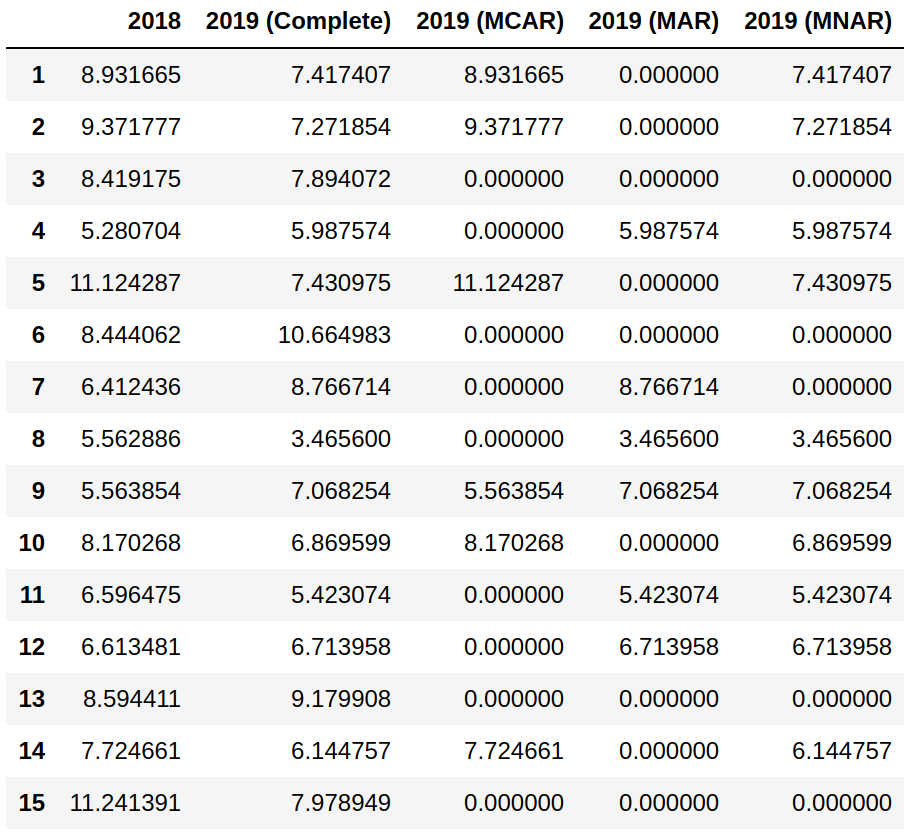
\includegraphics[width=\linewidth]{missingness}
		\caption{Different missingness mechanisms}
		\label{fig:miss1}
	\end{figure}
	
	In the MCAR scenario, we see a random spread of missing data, i.e. a random subset of those who answered the 2018 survey also answered the 2019 one. Things get more interesting in the next two columns. Suppose you are only interested in those who've slept less than 7.5 hours on average, so you only send a follow-up survey to those who reported less than 7.5 hours of sleep for 2018 (2018<7.5). This is MAR, since the missingness of the 2019 entries depends on the values for 2018. For the final column, suppose you sent out your 2019 survey to all the individuals who answered the 2018 one, but include a line stating "Only answer this survey if you slept less than 7.5 hours on average in 2019" (2019 < 7.5). This is MNAR, since the missingness of the 2019 entries depends on the values for those entries. Remember, the full dataset exists, but it has been censored due to some mechanism, in this case through your own design. 
	
	
	\section{The validity of missingness mechanisms}
	
	In controlled environemnts, like the one from the our example, we can guarantee that data are MAR since we control the censoring of the data (in this case by placing a cutoff between 2018 and 2019). However, it is rare that we have this much control over our data and a compelling reason to censor it so. In most real world scenarios we only have the data at hand to inform us about the missingnsess mechanism. Unfortunately, we cannot infer the missingness mechanism from data ...  We can check the validity of MCAR against MAR, but only under the unverifiable assumption that the data is not MNAR. Neither can we use the data at hand to support or refute on specific MNAR mechanism over another. The literature stresses the importance of sensitivity analyses in this case, checking the sensitivity of our inference under a variety of plausible assumptions. Finally MAR cannot be checked empirically against MNAR  (Cite from page 8, 9, and 10 in missing data). We therefore have to assume the missingness mechanism, most often MAR, and there are strong arguments for this. First and foremost is that assuming MAR yields good empirical results, which will be shown in later sections. %TODO Add more reasons for assuming MAR
	
	\section{What is imputation?}
	Imputation refers to substituting or ''filling in'' missing values with plausible estimates. The main strength of imputation is that it does not change the nature of the subsequent analysis. It makes it much easier for the data processor and analyst to work together since the processor's techniques won't interfere with the analysts'. Another benefit of imputation is that it augments the dataset, meaning that the dataset being analysed is larger than the original dataset, potentially yielding higher performance.
	
	
	\section{Techniques of interest}
	To properly evaluate the performance of MI, we should compare it to other similar and commonly used techniques, i.e. techniques that manipulate the dataset by either imputing or removing values. When choosing to apply a method it is important to keep two questions in mind. First, does the method under consideration give us consistent estimators for our model? Second, does the method give us appropriate measures of precision? How the following methods answer these questions is how we will decide the superiority of one method over another.
	
	\subsection{Ad hoc methods}
	Carpenter and Kenward (Missing data handbook) ...
	
	\textbf{Case deletion, also called complete case analysis (CCA):}
	A very common practice, CCA involves restricting analysis to entries with complete data. For those familiar with programming, a typical example would be to remove all rows from a dataframe with NaN entries. The first and most obvious problem with this approach is that it drastically reduces the amount of useable data. Additionally, this technique introduces large biases in the data if missingness is MAR or MNAR (CITE REVIEW PAPER FROM TURID). Only under MCAR is the data not biased when conducting CCA, but one is still faced with reduced accuracy due to missing data. 
	
	
	\textbf{Mean imputation:}
	
	\textbf{Hot Deck imputation:}
	
	\subsection{Statistically principled methods}
	
	
	\textbf{Single imputation}
	
	
	Maximum likelihood and mixed linear models... This is the current alternative to the main method which we will discuss in the next chapter, multiple imputation. MI is often preferred over ML and MLM for two reasons: 
	1. It often performs similarly to multiple imputation with only a small advantage on certain kinds of data.
	2. It is less easy to use for non-statisticians
	A
	
	\section{Multiple imputation}
	
	Highly robust technique that yields gains even with relatively small portions of missing data. 
	
	Only become feasible in the last 20 years due to computing power required.
	
	Bayesian approach.
	
	Between imputation variance
	
	
	
	
	\subsection{Specifying the imputation model}
	
	\subsection{Rubin's rules}
	
	\subsection{Potential pitfalls}
	When there is missing data in several variables of different types ,for example continuous and binary, and the data is structured, specifying the imputation model can be quite difficult. This is because it has to be a joint model...
	
	
	
	\subsection{When to use multiple imputation?}
	Computational resources and time to create the full joint imputation model. (Handbook 236)
	
	A common measure used to decide when to use multiple imputation is percentage of missing data.
	
	However, Madley-Dowd et. al. (Proportion of missing data paper) propose a different measure.
	
	MI can be used to perform sensitivity analysis by varying the imputation model.
	
	\section{Experiments}
	In this section we will use Madley-Dowd et. al.'s missingness measure to...
	
	\subsection{Synthetic example}
	
	"The MCAR missingness mechanism
	removed the first p observations such that pn gives the
	required proportion of missing data. MAR missingness
	was simulated under a logistic regression model using
	
	The value of a was manipulated for the different simu-
	lation settings to provide the required proportion of missing
	data on average across data sets." from (P. Madley-Dowd et a)
	
	Also check out their motivation for the generating of the data
	
	\subsubsection{Inference}
	Test statistics
	Different tests
	
	\subsubsection{Prediction}
	
	\subsubsection{Classification}
	
	\subsection{Performance across different data types}
	Continuous
	Categorical (binary, multicategory)
	Time to event
	Timeseries
	
	\subsection{Sensitivity analysis}
	
	\subsection{Real data}
	
	Description of the data
	
	HUNT Norwegian data
	
	Andreas data webSite
	balanced number of classes for classification
	
	
	\subsection{TODO}
	Difference between baysian and frequentist paradigm.
	Citation example:
	\cite[P.10]{grund_pooling_2016}.

	\bibliography{bib3}	
	\bibliographystyle{apalike}
	
\end{document}
